\documentclass{beamer}

\usepackage{graphicx,wrapfig,lipsum}
%\graphicspath{ {images_latex/} }

%\setbeamertemplate{background canvas}{
\includegraphics[width=\paperwidth-100, height=\paperheight]{images_latex/foto.jpg}}

\useoutertheme{infolines}
\usetheme{Hannover}


\title{MyRoute}



%\subtitle { \vspace{1cm} \color{black}Juan Germ\'an G\'omez G\'omez \\ \'Alvaro L\'opez Jim\'enez \\ Antonio Jos\'e Camarero Ortega \\ Rub\'en Mar\'in Asunci\'on \\ Rub\'en Mogica Garrido \\ Alejandro Ru\'iz Becerra \\ Valent\'in Pedrosa Campoy}

\date{18/01/2019}

\subject{Prácticas DGP}
% This is only inserted into the PDF information catalog. Can be left
% out.

% Delete this, if you do not want the table of contents to pop up at
% the beginning of each subsection:
\AtBeginSubsection[]
{
  \begin{frame}<beamer>{}
    \tableofcontents[currentsection,currentsubsection]
  \end{frame}
}

\begin{document}

\begin{frame}
  \titlepage 
\end{frame}

\begin{frame}{\'Indice}
  \tiny 
  \tableofcontents
  % You might wish to add the option [pausesections]
\end{frame}

% Section and subsections will appear in the presentation overview
% and table of contents.
\section{Gesti\'on del Equipo y del Proyecto}

\subsection{Organizaci\'on del Equipo}

\begin{frame}{Organizaci\'on}{Objetivos de cada iteraci\'on}
  \begin{tabular}{cll}
  Iteraci\'on  & Objetivos & Organizaci\'on \\\hline \\
  1  &  An\'alisis Etnogr\'afico,  & Todos \\
     &  Dise\~no visual            & Dise\~no\\[0.3cm]
  2  &  Prototipo  & Backend, Frontend \\[0.3cm]
  3  &  Funcionalidad & Dise\~no, Backend, Frontend
  \end{tabular}
\end{frame}


% Iteración 1
\begin{frame}{Organizaci\'on}{Iteraci\'on 1}
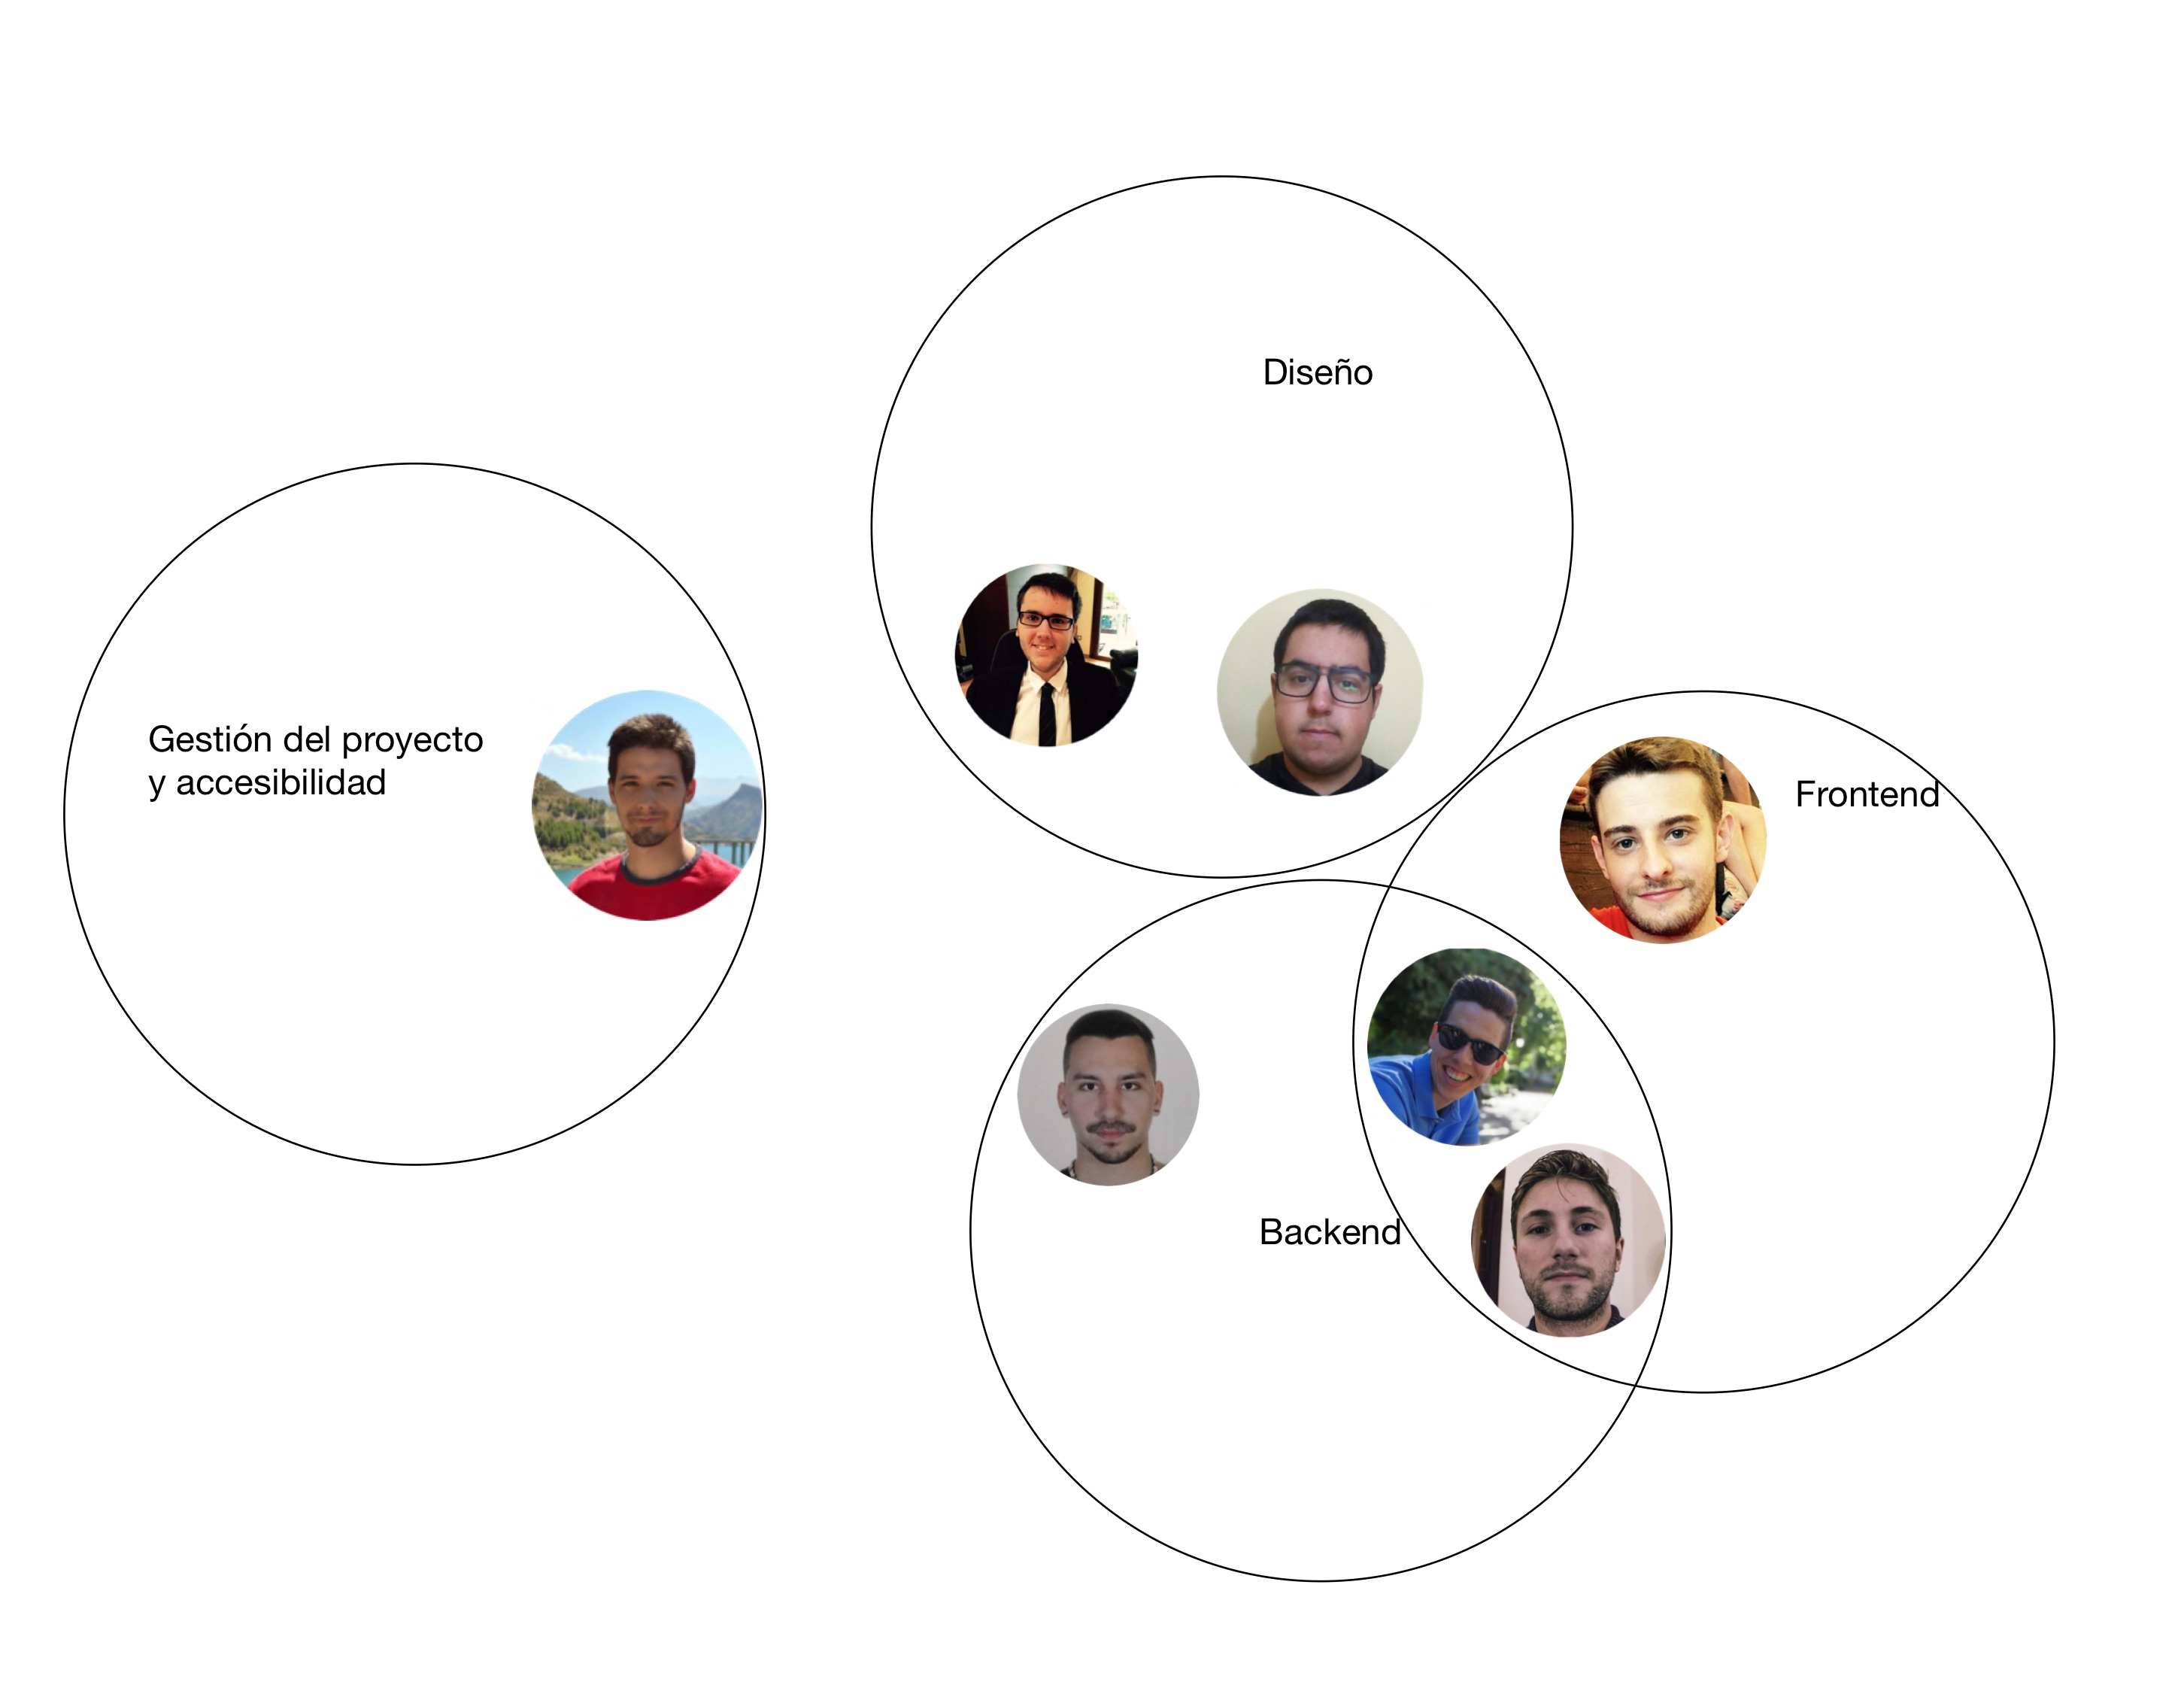
\includegraphics[scale=0.1]{images_latex/org_itr1}
\end{frame}

\begin{frame}{Tareas}{Iteraci\'on 1, (18 tareas)\\
 An\'alisis Etnogr\'afico y Dise\~no.}
\centering
\hspace{1cm}
\\[1cm]
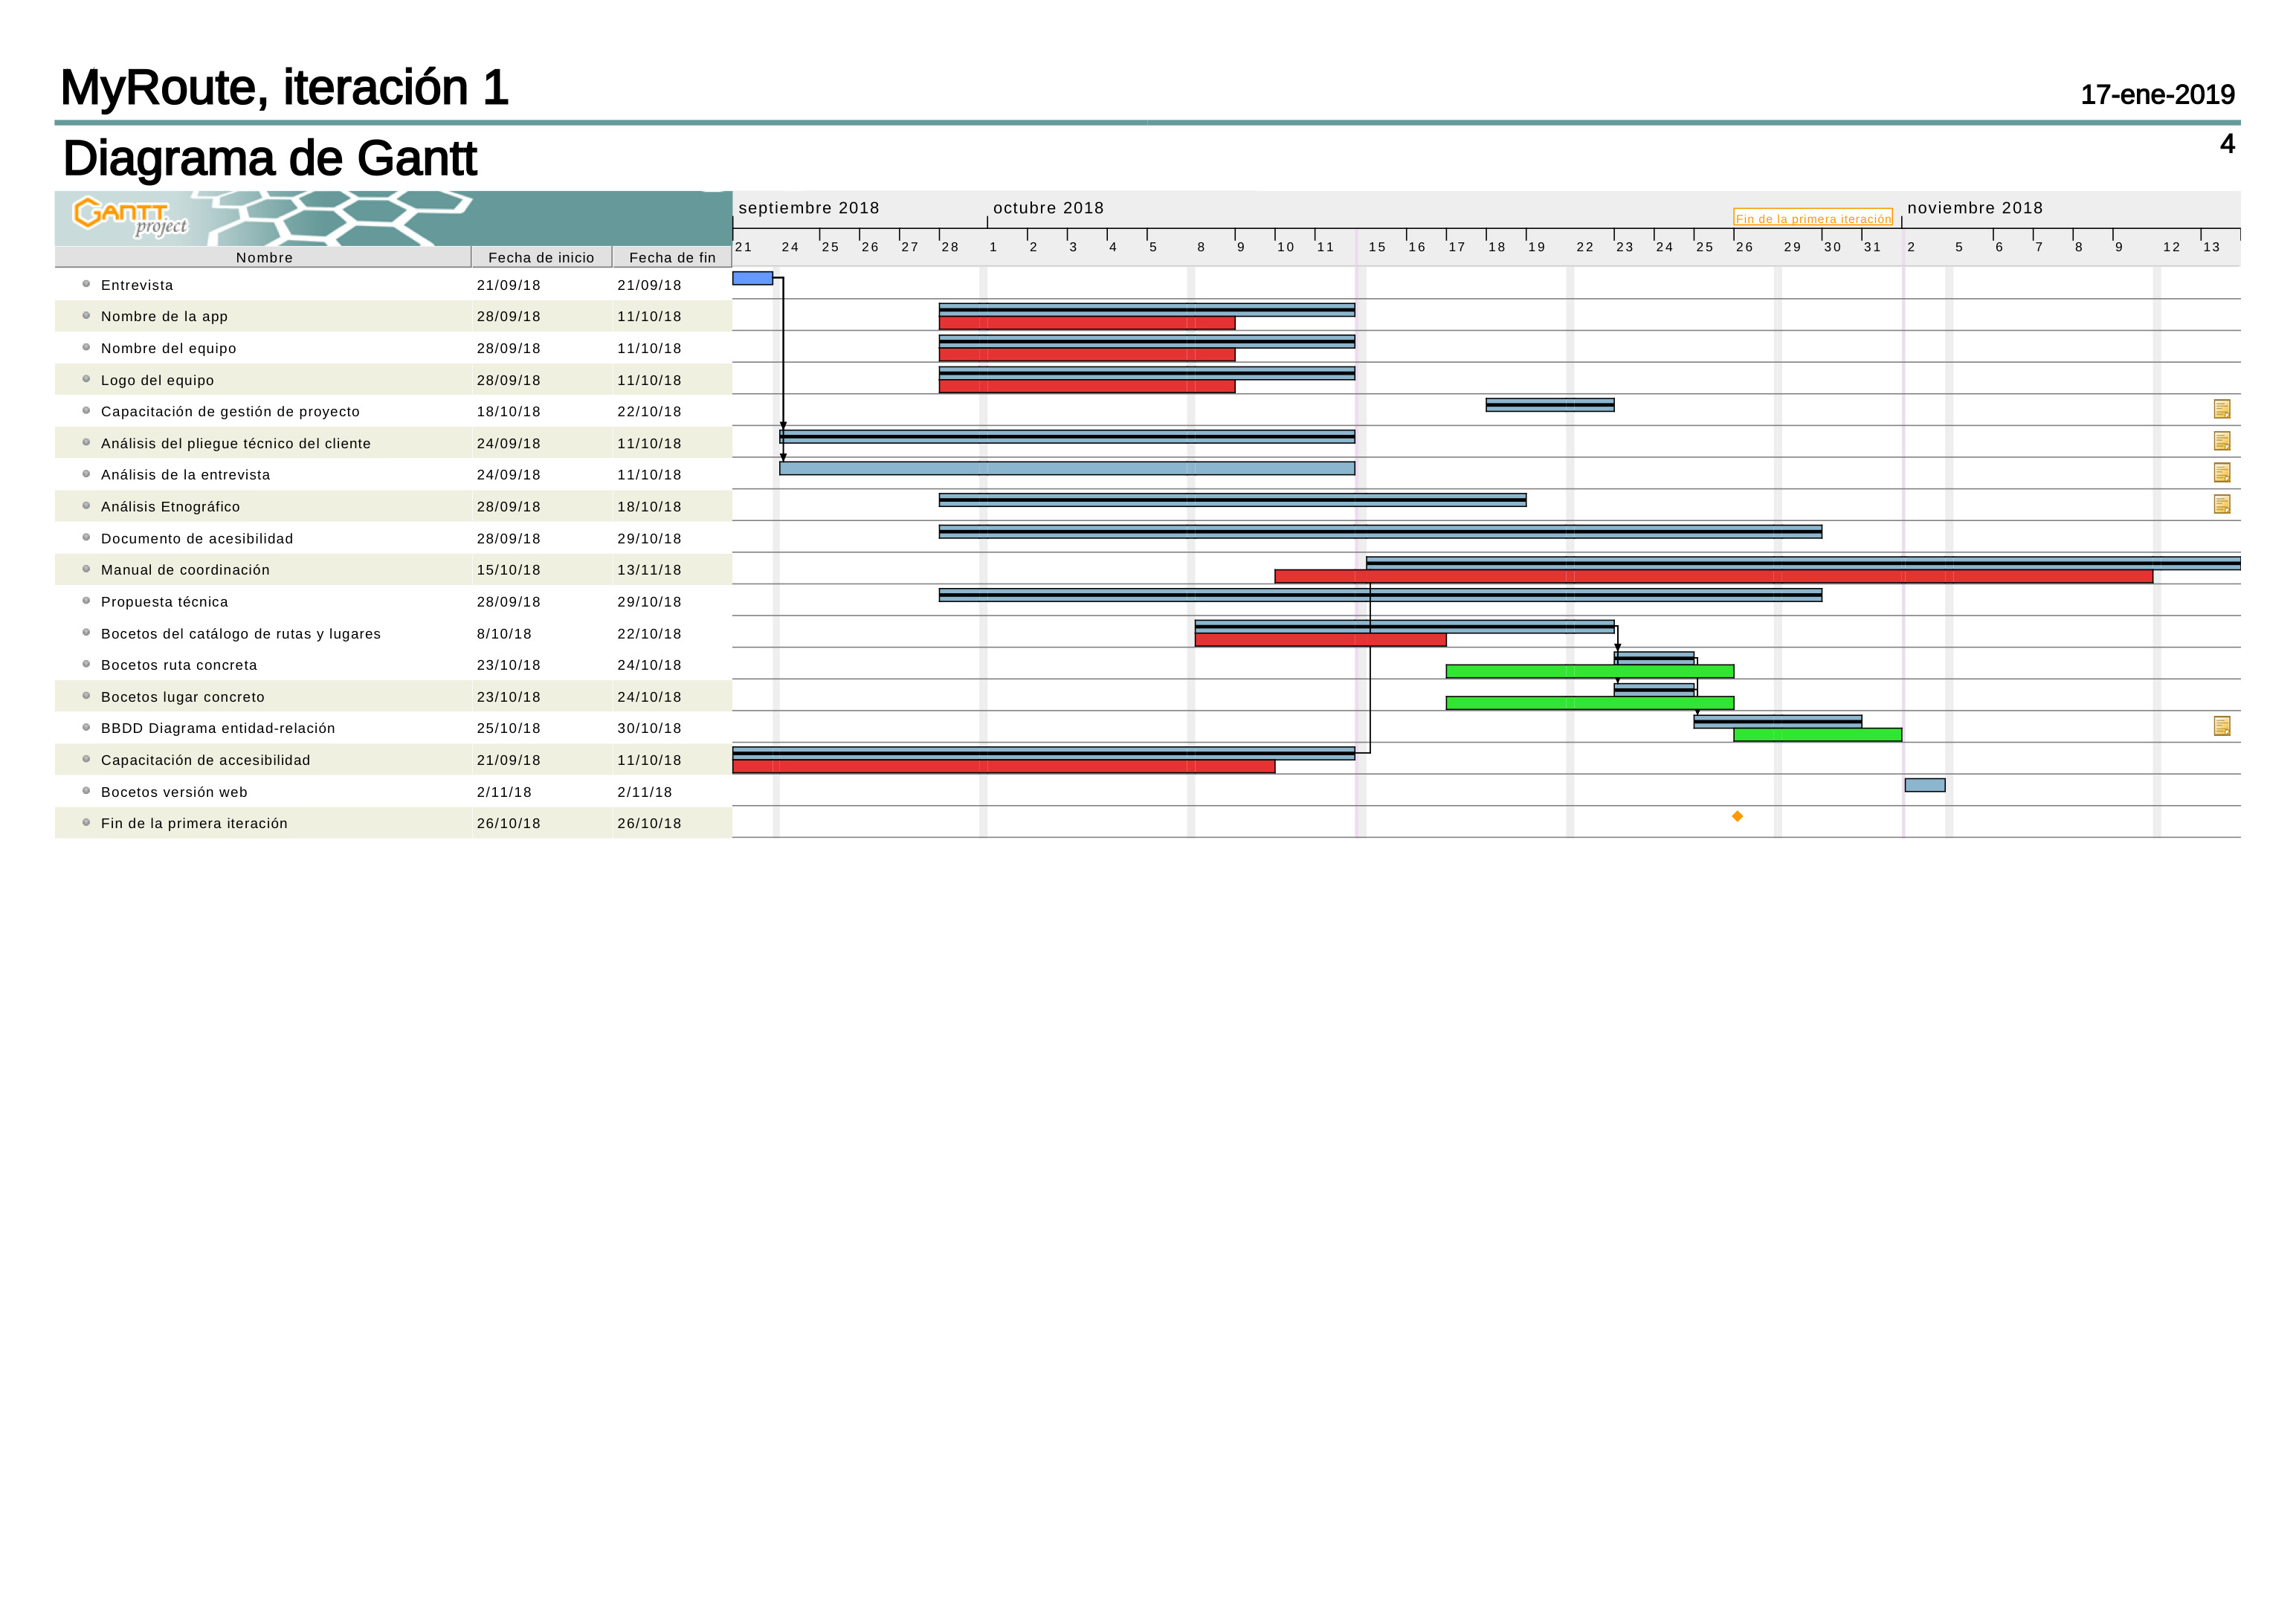
\includegraphics[width=0.8\paperwidth]{images_latex/gantt_itr1}

\end{frame}



%Iteración 2
\begin{frame}{Organizaci\'on}{Iteraci\'on 2}
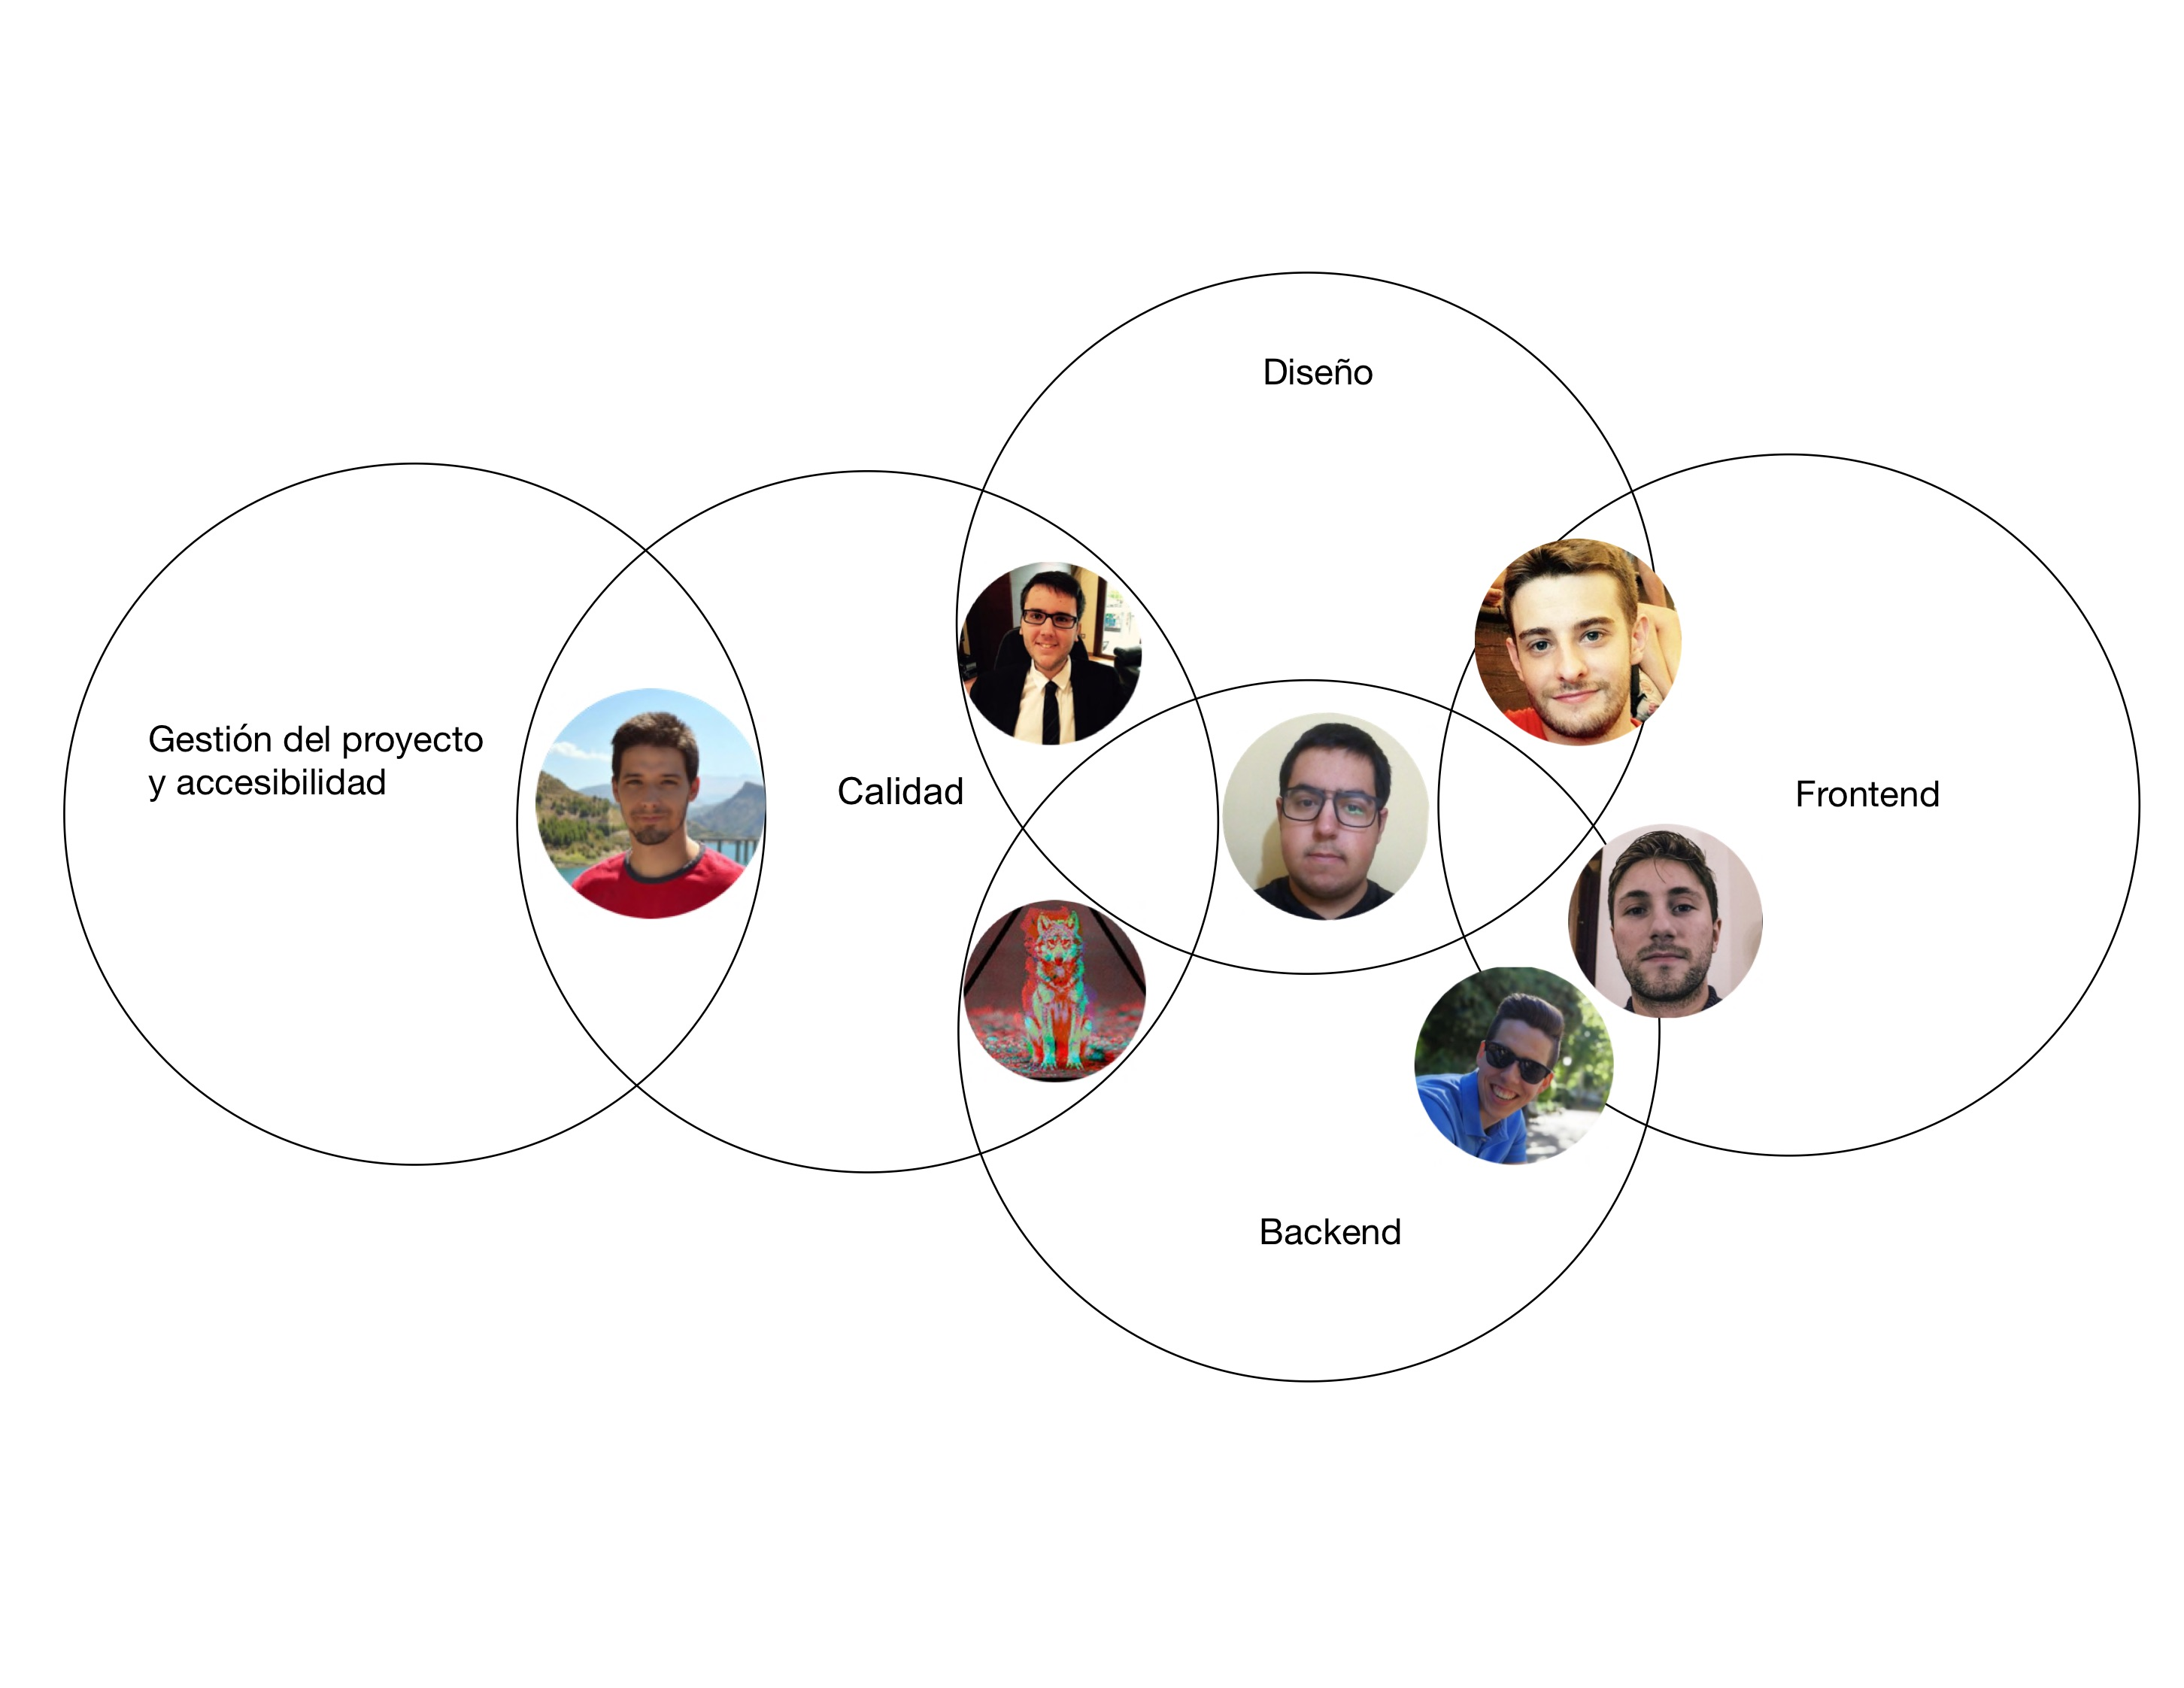
\includegraphics[scale=0.1]{images_latex/org_itr2}
\end{frame}

\begin{frame}{Tareas}{Iteraci\'on 2, (9 plan, 4 no plan)\\
Prototipo}
\centering
\hspace{1cm}
\\[1cm]
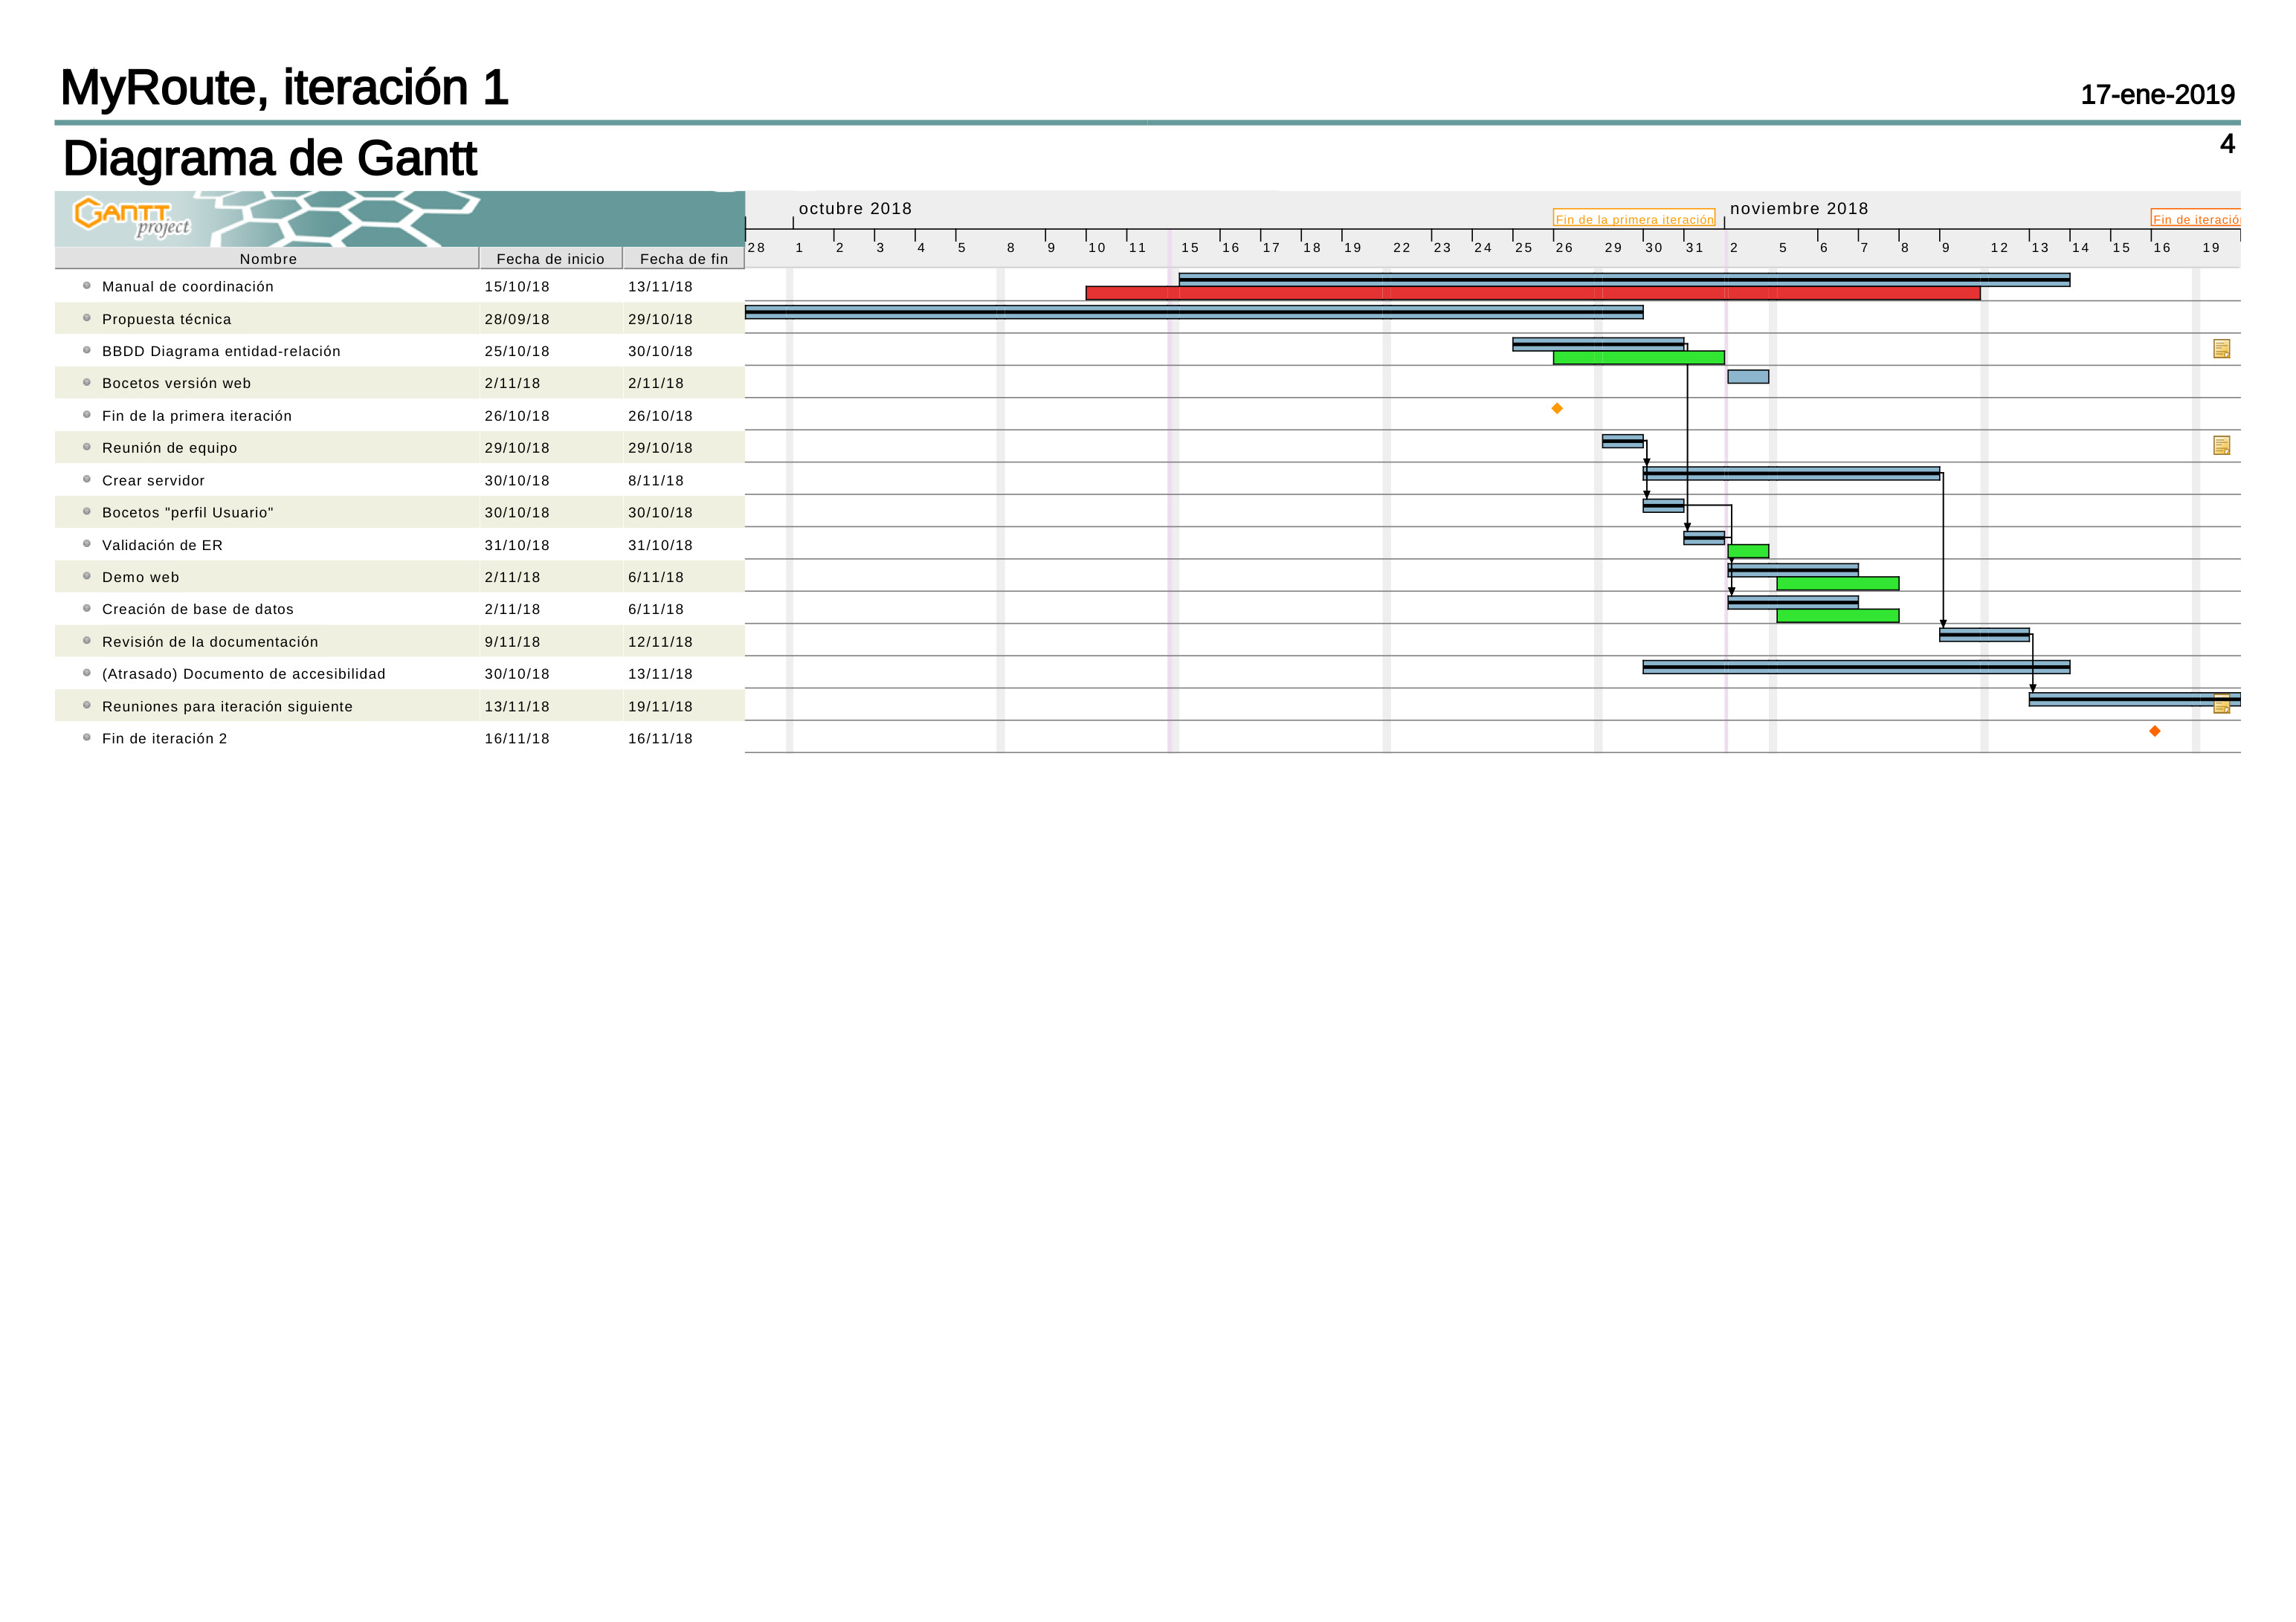
\includegraphics[width=0.8\paperwidth]{images_latex/gantt_itr2}
\end{frame}



%Iteración 3
\begin{frame}{Organizaci\'on}{Iteraci\'on 3}
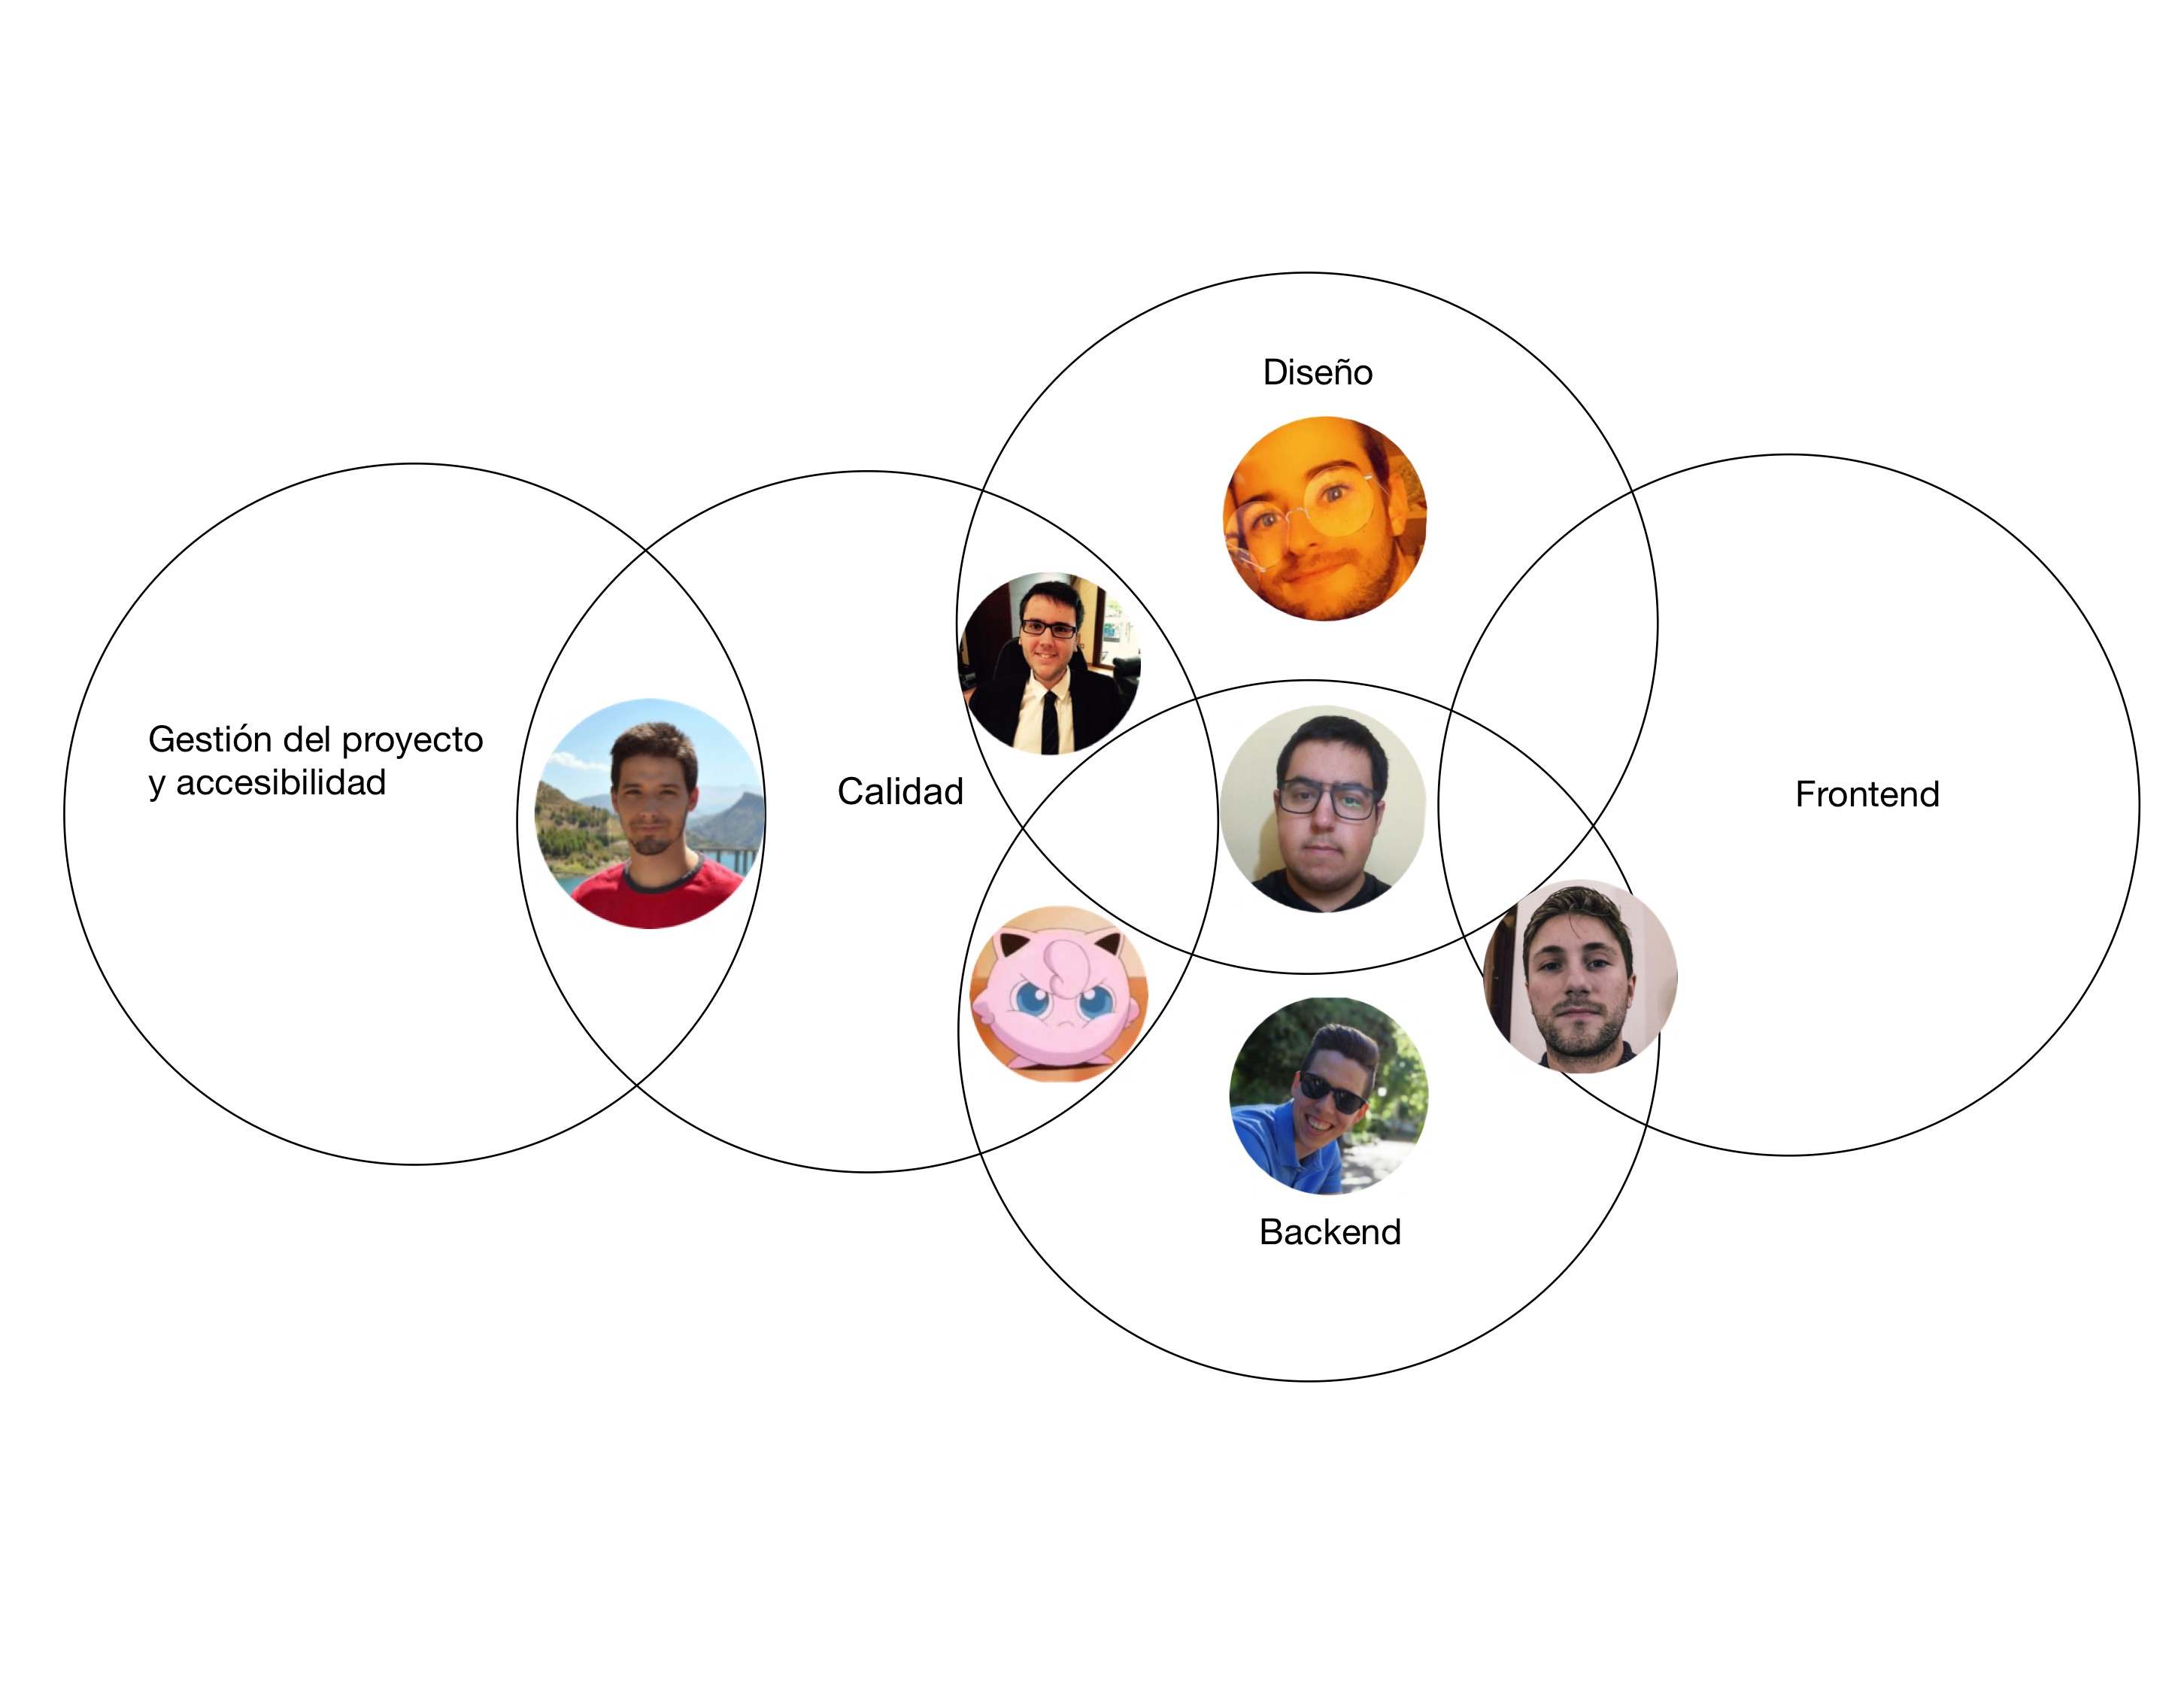
\includegraphics[scale=0.1]{images_latex/org_itr3}
\end{frame}

\begin{frame}{Tareas}{Iteraci\'on 3, (72 plan, 4 no plan)\\
Funcionalidad}
\centering
\hspace{1cm}
\\[1cm]
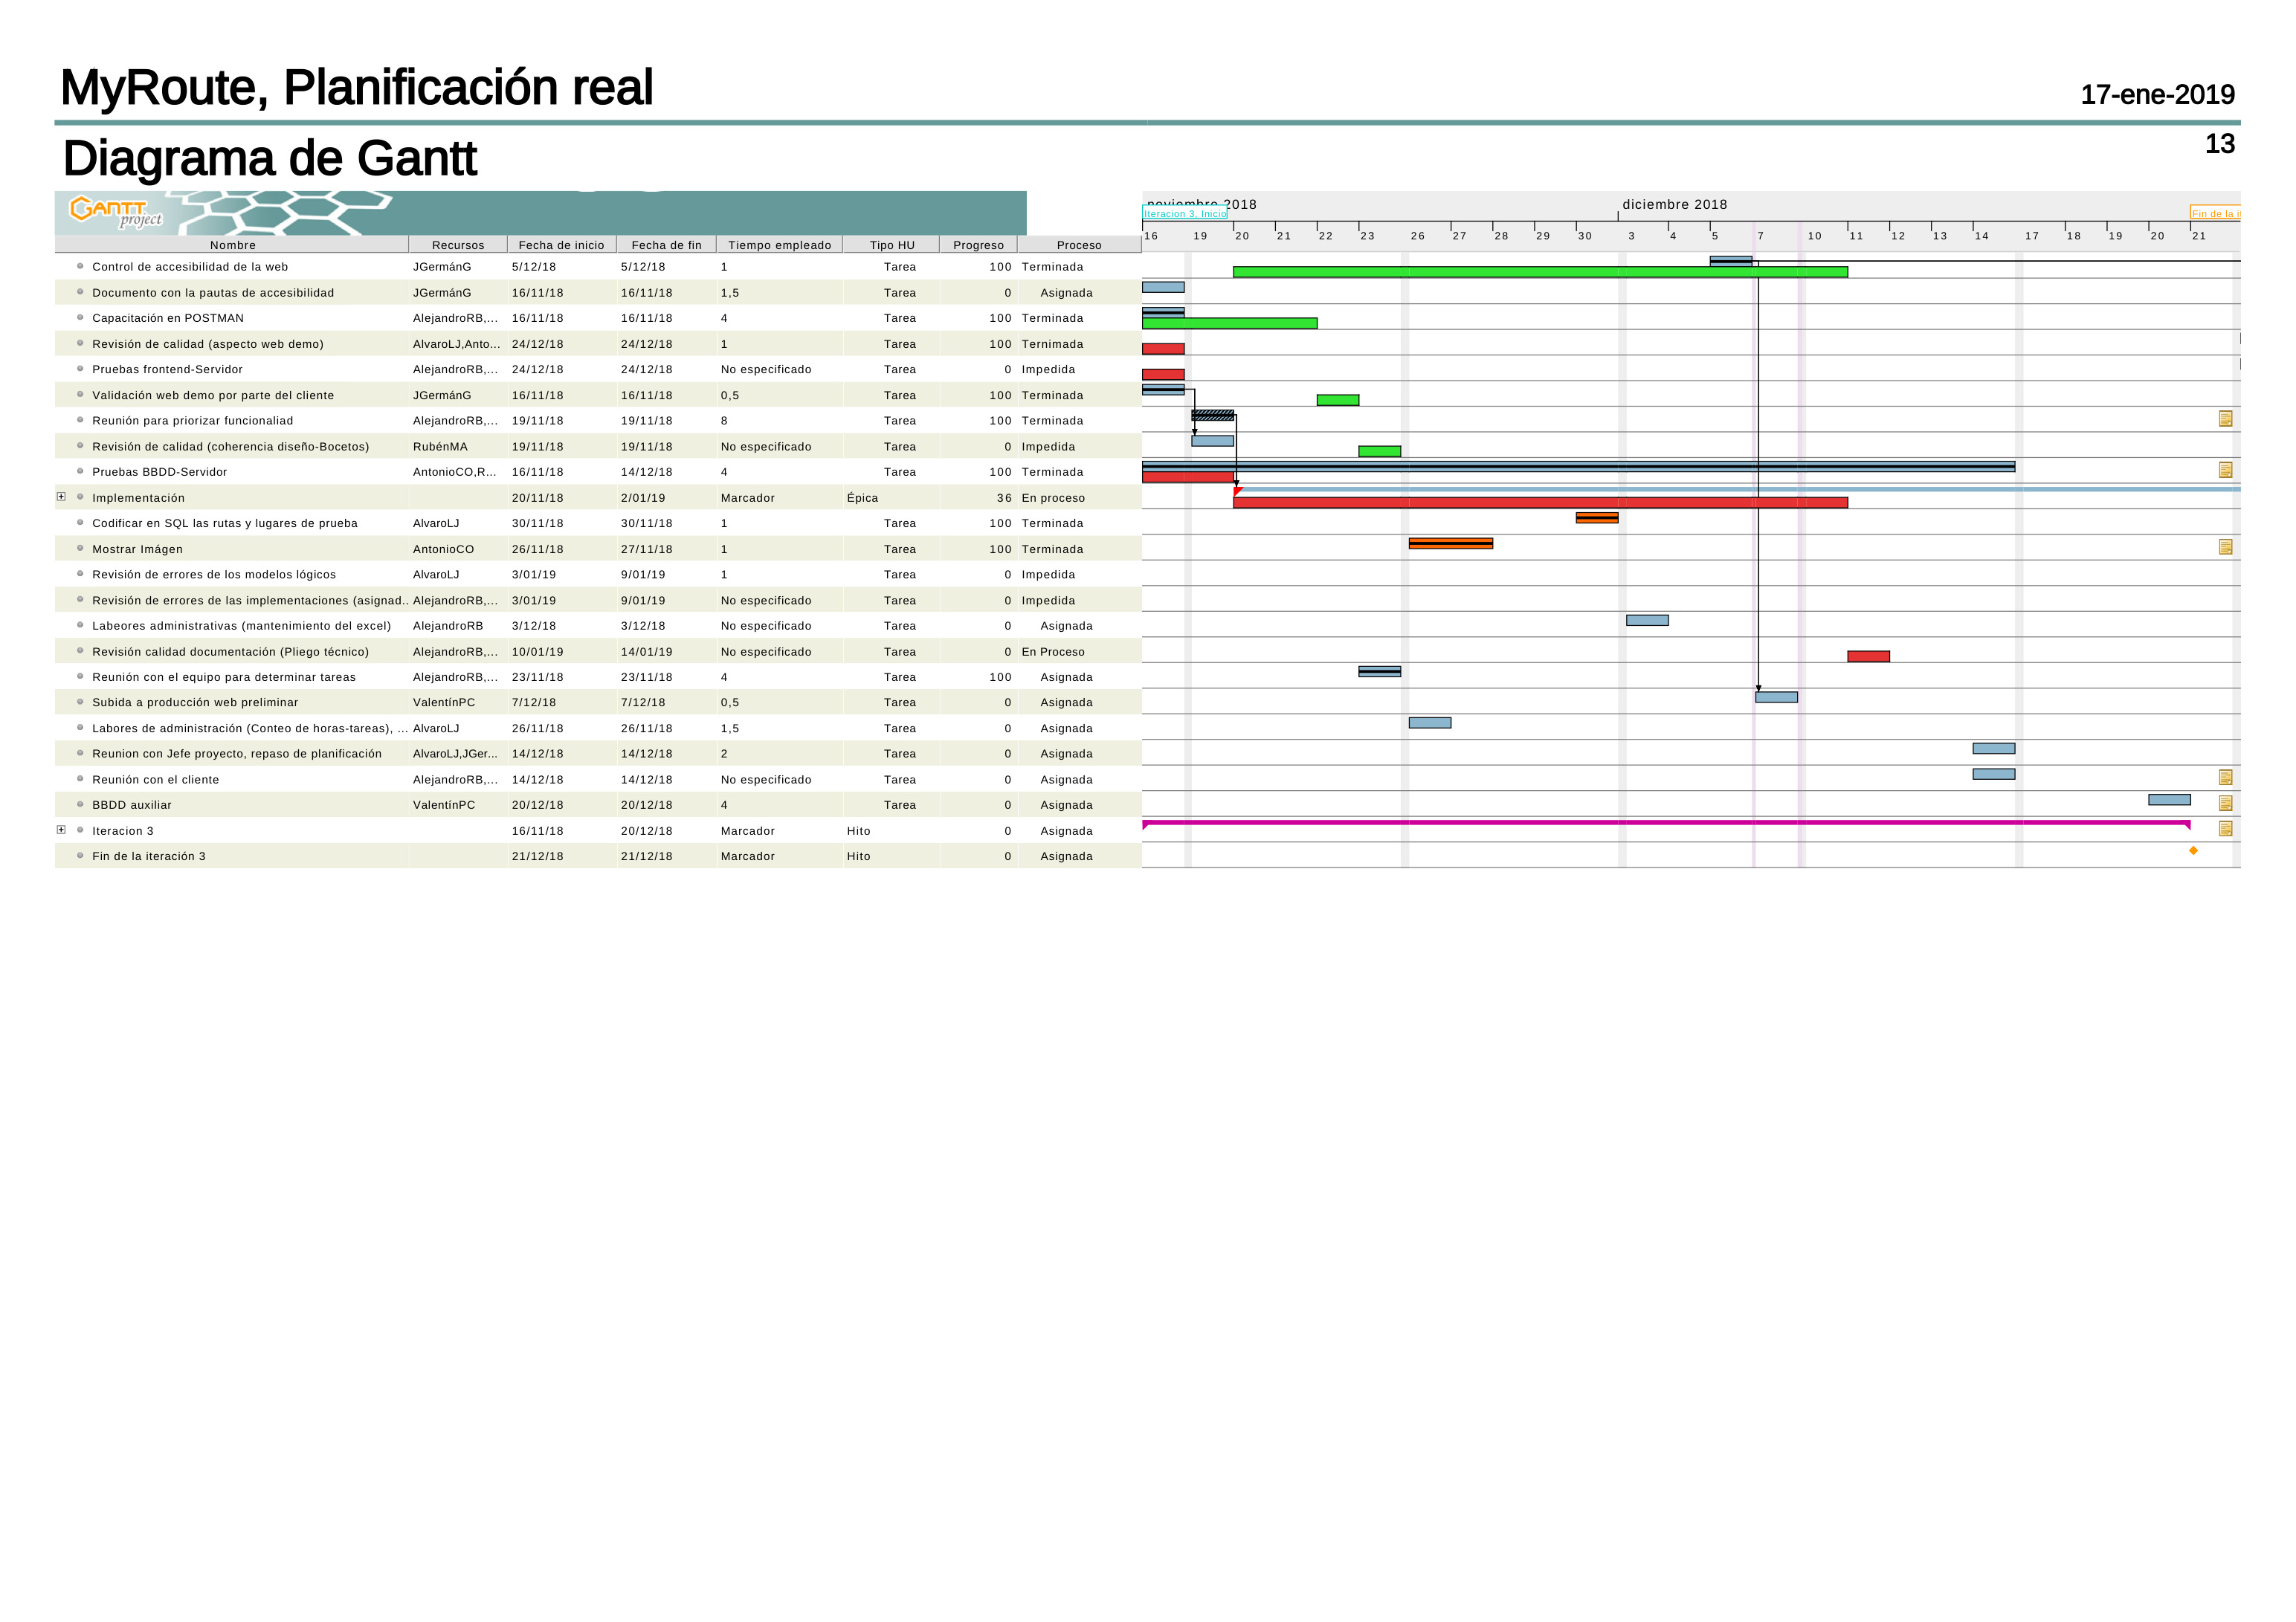
\includegraphics[width=0.8\paperwidth]{images_latex/gantt_itr3}
\end{frame}

%Accesibilidad
\subsection{Accesibilidad}
\begin{frame}{Accesibilidad}{ONCE, W3C}
  \begin{figure}
   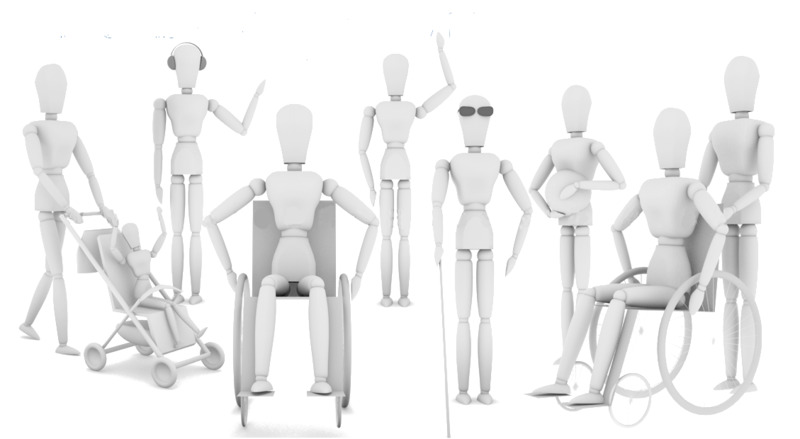
\includegraphics[scale=0.3]{images_latex/accesibilidad}
  \end{figure}

\end{frame}


\subsection{Comunicaci\'on}

\begin{frame}{Comunicaci\'on Externa}
	\begin{figure}[H]
	\centering
	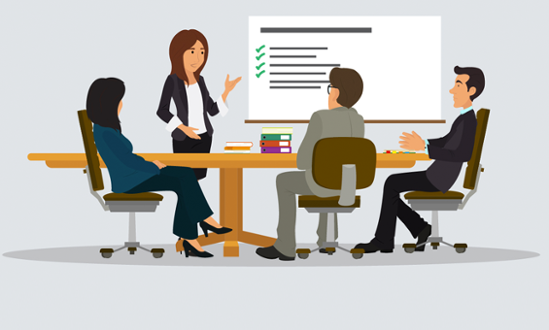
\includegraphics[width=0.35\paperwidth, height=0.4\paperheight]{images_latex/reuniones} 
	\hspace{0.7cm}
	
\includegraphics[width=0.35\paperwidth, height=0.4\paperheight]{images_latex/entrega}
	\end{figure}

\end{frame}

\begin{frame}{Comunicaci\'on Interna}
	\begin{figure}[H]
	\centering
	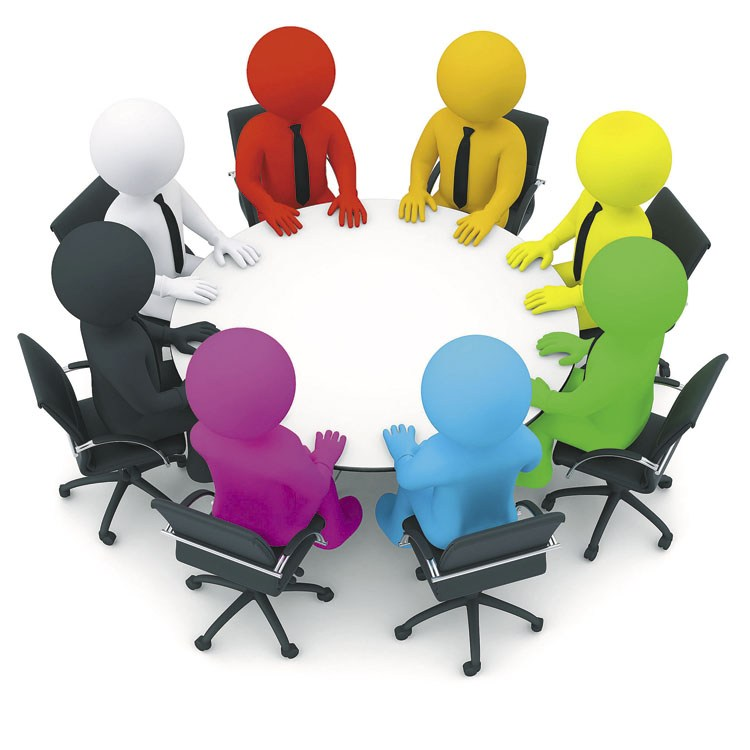
\includegraphics[width=0.35\paperwidth, height=0.4\paperheight]{images_latex/reuniones2}
	\hspace{0.7cm}
	
\includegraphics[width=0.35\paperwidth, height=0.4\paperheight]{images_latex/telegram}
	
\includegraphics[width=0.35\paperwidth, height=0.4\paperheight]{images_latex/drive}
	\hspace{0.7cm}
	
\includegraphics[width=0.35\paperwidth, height=0.4\paperheight]{images_latex/github}
	\end{figure}

\end{frame}

\subsection{Seguimiento}
	% Tabla general	
	\begin{frame}{Seguimiento}{Control de horas}
	\centering
	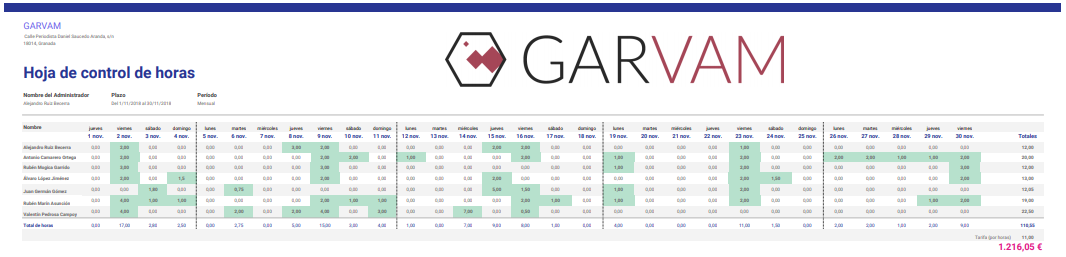
\includegraphics[width=0.8\paperwidth]{images_latex/seguimiento/tabla_horas}
	\end{frame}

	% Tabla general ampliada	
	\begin{frame}{Seguimiento}{Control de horas}
	\centering
	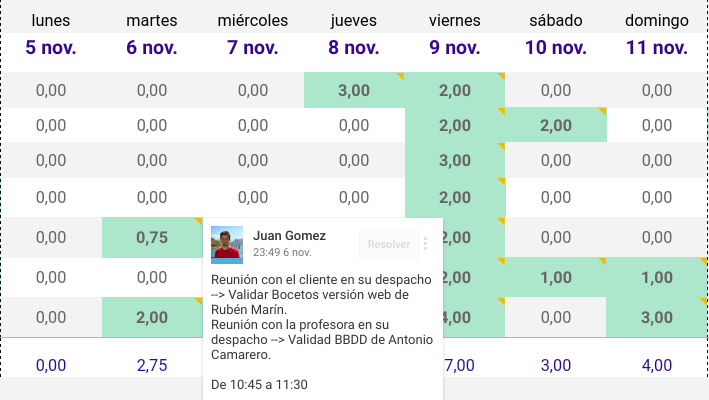
\includegraphics[width=0.8\paperwidth]{images_latex/seguimiento/tabla_horas_zoomed}
	\end{frame}

	% Estadísticas general	
	\begin{frame}{Seguimiento}{Estad\'isticas mensuales}
	\centering
	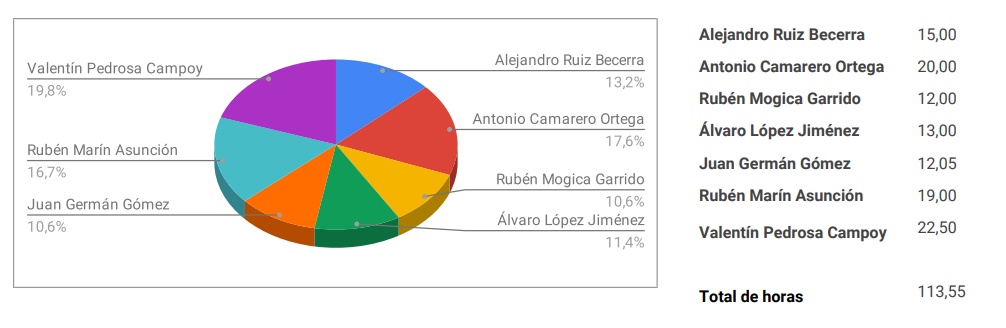
\includegraphics[width=0.8\paperwidth]{images_latex/seguimiento/graf_horas_1}
	\end{frame}

	% Estadística semanal 1
	\begin{frame}{Seguimiento}{Estad\'isticas semanales}
	\centering
	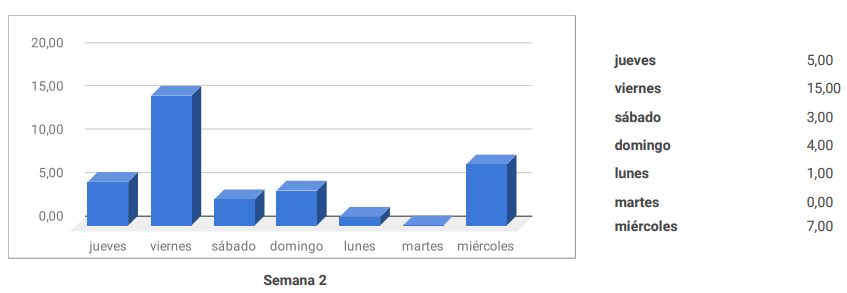
\includegraphics[width=0.8\paperwidth]{images_latex/seguimiento/graf_horas_2}
	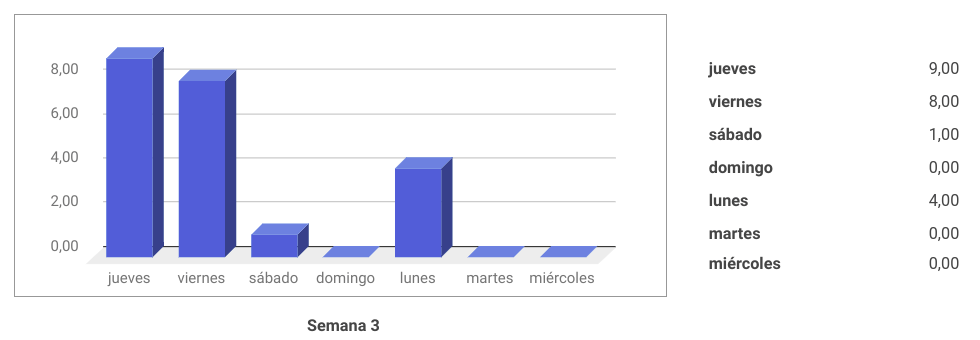
\includegraphics[width=0.8\paperwidth]{images_latex/seguimiento/graf_horas_3}
	\end{frame}

%\section{Gesti\'on del Proyecto}

%\subsection{Tareas realizadas en cada iteraci\'on}

\subsection{Gesti\'on de la calidad}
	\begin{frame}{Gesti\'on de la calidad}
		\begin{itemize}
			\item {
				Validar requisitos con el cliente.
			}
			\item {
				Bocetos iniciales valorados por todo el equipo.
			}
			\item {
				Cambios propuestos consultados con el cliente. Abiertos a cr\'iticas.
			}
			\item {
				Pruebas por separado de back-end y front-end.
			}
			\item {
				Funcionalidad implementada = funcionalidad probada.
				
			}
		\end{itemize}
		
		
		\begin{figure}
			%\hspace{0.3cm}
    		
\includegraphics[width=0.4\textwidth, height=0.5\textheight]{images_latex/conversacion}
    		\hspace{0.7cm}
    		
\includegraphics[width=0.5\textwidth, height=0.5\textheight]{images_latex/testing}
		\end{figure}
	
	\end{frame}

\section{Arquitectura y tecnolog\'ia}

\subsection{Arquitectura del sistema}

	\begin{frame}{Arquitectura del sistema}
		\begin{itemize}
			\item {
				Back-end : API REST.
				
			}
			\item {
				Front-end : SPA (Single Page Application).
			}
			\item {
				Base de datos : Relacional.
				%\begin{wrapfigure}{r}{0cm}
				%
\includegraphics{images_latex/postgresql}
				%\end{wrapfigure} 
				%
\includegraphics[scale=0.1]{images_latex/postgresql}
				
			}
		\end{itemize}
		
		
		\begin{figure}[h]
			%\hspace{0.3cm}
    		\centering
    		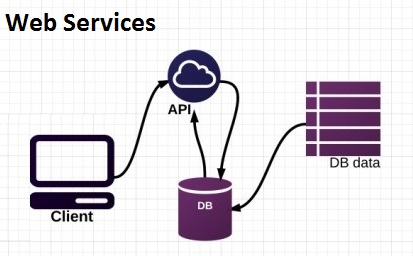
\includegraphics[width=0.6\textwidth, height=0.4\textheight]{images_latex/rest-api}

		\end{figure}
		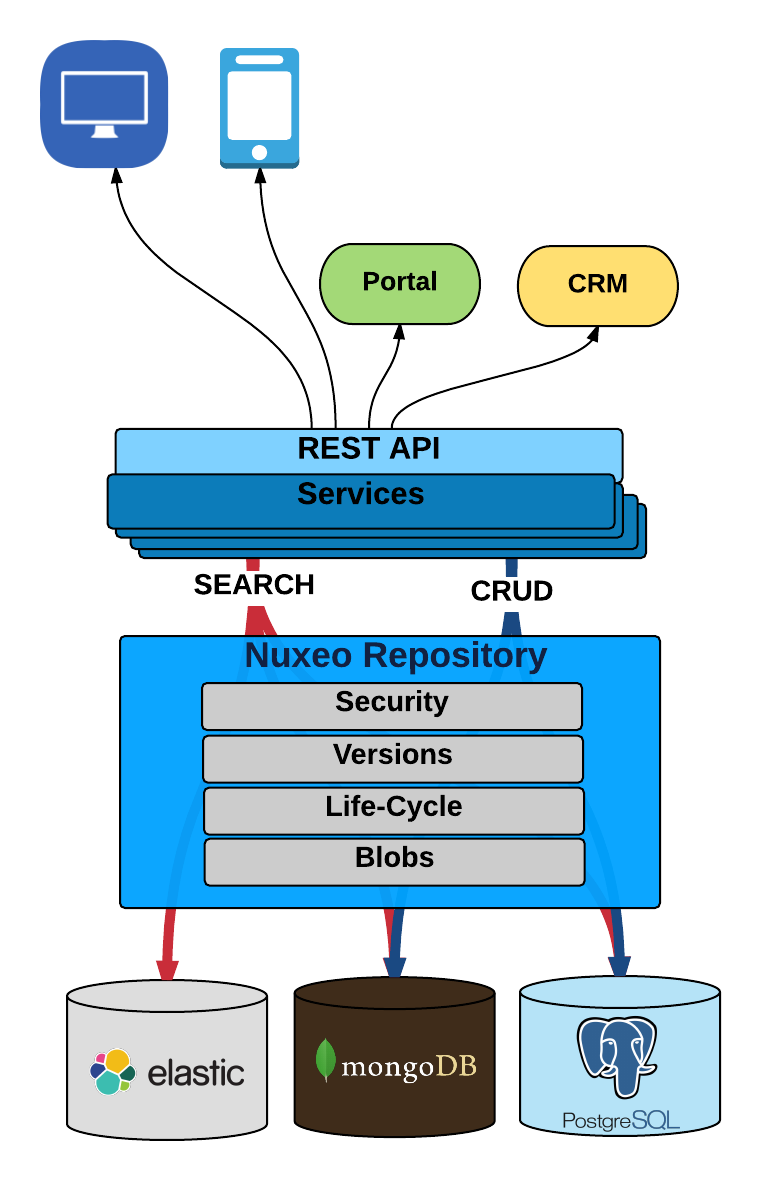
\includegraphics[scale=0.1]{images_latex/api}
	
	\end{frame}

\subsection{Herramientas y tecnolog\'ia}
\begin{frame}{Herramientas y tecnolog\'ia}
		\begin{figure}[H]
	\centering
	
\includegraphics[width=0.35\paperwidth, height=0.3\paperheight]{images_latex/laravel}
	\hspace{0.1cm}
	
\includegraphics[width=0.35\paperwidth, height=0.2\paperheight]{images_latex/angular}
	\centering
	
\includegraphics[width=0.4\paperwidth, height=0.35\paperheight]{images_latex/postgresql-nombre}
	\end{figure}
	
	\end{frame}

\section{Pliego T\'ecnico}

\subsection{Cumplimiento del Pliego}

\subsection{Valor A\~nadido}

\section{Retrospectiva}

\subsection{An\'alisis DAFO}

\begin{frame}{An\'alisis DAFO}
	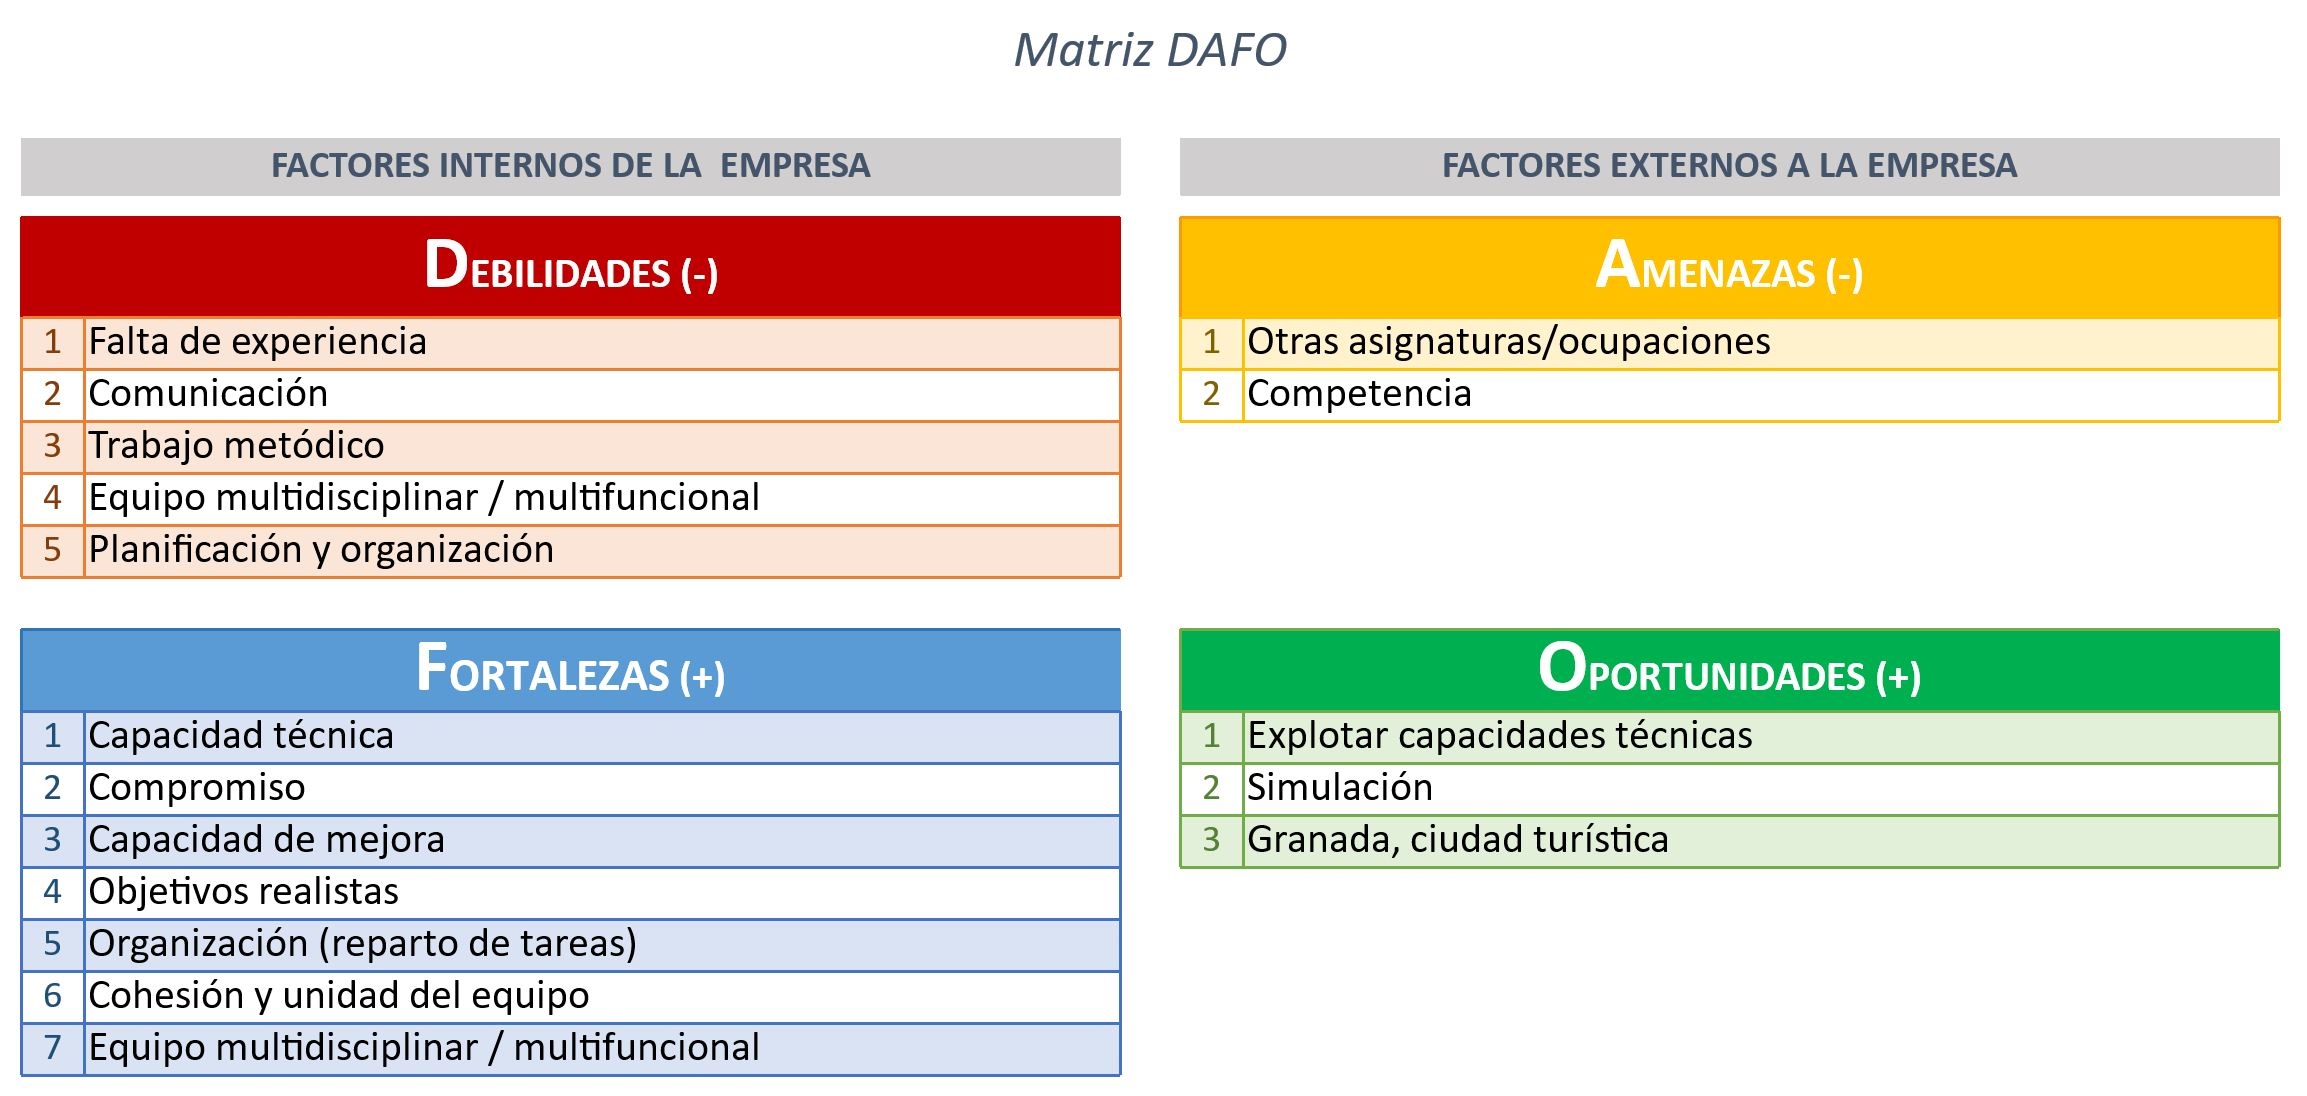
\includegraphics[width=0.8\paperwidth, height=0.8\paperheight]{images_latex/DAFO}
	  
\end{frame}

\subsection{Lecciones aprendidas}

\subsection{Autocr\'itica y cr\'itica a la asignatura}

\begin{frame}{Autocr\'itica}
  \begin{itemize}
  \item { Buen trabajo y buenos resultados. }
  \item { Aspectos a mejorar de cara a futuros proyectos como equipo:
    \begin{itemize}
    \item {Mejorar la comunicaci\'on}
    \item {Ser m\'as met\'odicos}
    \item {Mejorar las habilidades t\'ecnicas de algunos miembros}
    \item {Mejorar la organizaci\'on para evitar bloqueos}
    \end{itemize}
  }
  \end{itemize}
\end{frame}

\begin{frame}{Cr\'itica a la asignatura}
  \begin{itemize}
  \item { ?`C\'omo se gestiona un equipo?}
  \item { ?`C\'omo se gestiona un proyecto?}
  \item {?`C\'omo es trabajar en equipo?}
  \end{itemize}
  
    \begin{itemize}
    \item {No existe jerarqu\'ia}
    \item {Libertad del proyecto y falta de experiencia conlleva confusi\'on}
    \end{itemize}
    
\end{frame}

\subsection{Valoraci\'on Final}

\begin{frame}{Valoraci\'on Final}
	\begin{itemize}
 	 \item {
  		Aprender a organizarnos.
 	 }
 	 \item {
  		Entorno de trabajo realista.
 	 }
 	 \item {
		C\'omo trabajar en un grupo grande.
 	 }
 	 \item {
  		Afrontar problemas no previstos.
 	 }
 	 
	
\includegraphics[width=0.3\textwidth, height=0.5\textheight]{images_latex/valoracion}
		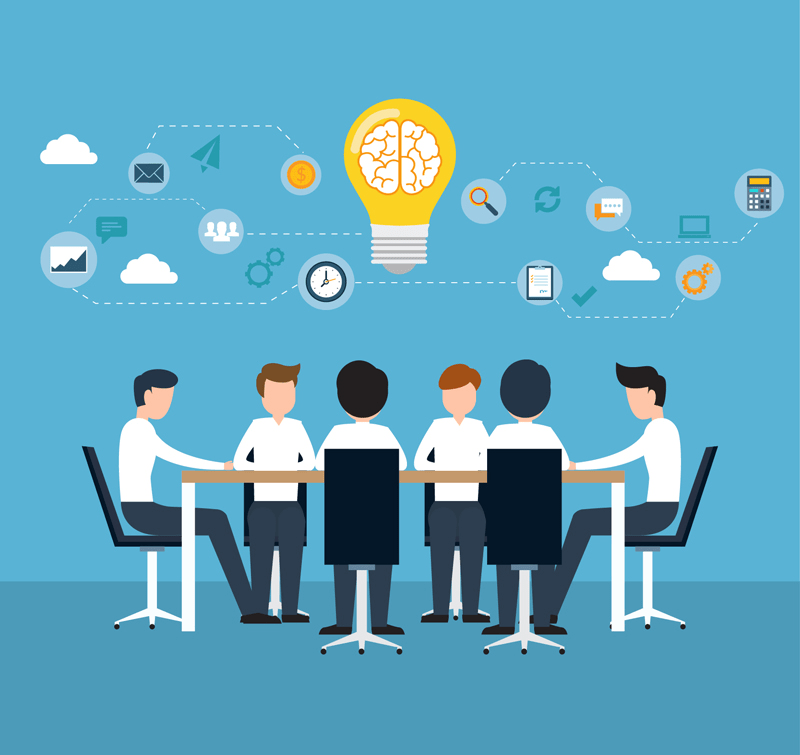
\includegraphics[width=0.5\textwidth, height=0.45\textheight]{images_latex/trabajoequipo}
  \end{itemize}
\end{frame}

\begin{frame}{Mejoras}
	\begin{itemize}
 	 \item {
  		Mejor organización inicial.
 	 }
 	 \item {
  		Plantear mejor las decisiones a largo plazo.
 	 }
 	 \item {
		Tener planes ante improvistos
 	 }
 	
  \end{itemize}
  	\begin{figure}[H]
  		
\includegraphics[width=0.7\textwidth, height=0.5\textheight]{images_latex/largoplazo}
  	\end{figure}
\end{frame}

\begin{frame}{Gracias}
	\centering
	
\includegraphics[width=0.6\paperwidth, height = 0.2\paperheight]{images_latex/logo}
\end{frame}


% You can reveal the parts of a slide one at a time
% with the \pause command:
%\begin{frame}{Second Slide Title}
%  \begin{itemize}
%  \item {
%    First item.
%    \pause % The slide will pause after showing the first item
%  }
%  \item {
%    Second item.
%  }
  % You can also specify when the content should appear
  % by using <n->:
%  \item<3-> {
%    Third item.
%  }
%  \item<4-> {
%    Fourth item.
%  }
  % or you can use the \uncover command to reveal general
  % content (not just \items):
%  \item<5-> {
%    Fifth item. \uncover<6->{Extra text in the fifth %item.}
%  }
%  \end{itemize}
%\end{frame}




\end{document}